\documentclass{article}

\usepackage{graphicx}
\usepackage{tikz}
\usepackage{tikzsymbols}
\usetikzlibrary{calc,patterns,shapes.geometric}
\pagestyle{empty}
\usepackage[margin=0pt]{geometry}
\geometry{papersize={14in,12in}}

\def\centerarc[#1](#2)(#3:#4:#5){\draw[#1] ($(#2)+({#5*cos(#3)},{#5*sin(#3)})$) arc (#3:#4:#5);}

\begin{document}
	\begin{figure}
		\centering
		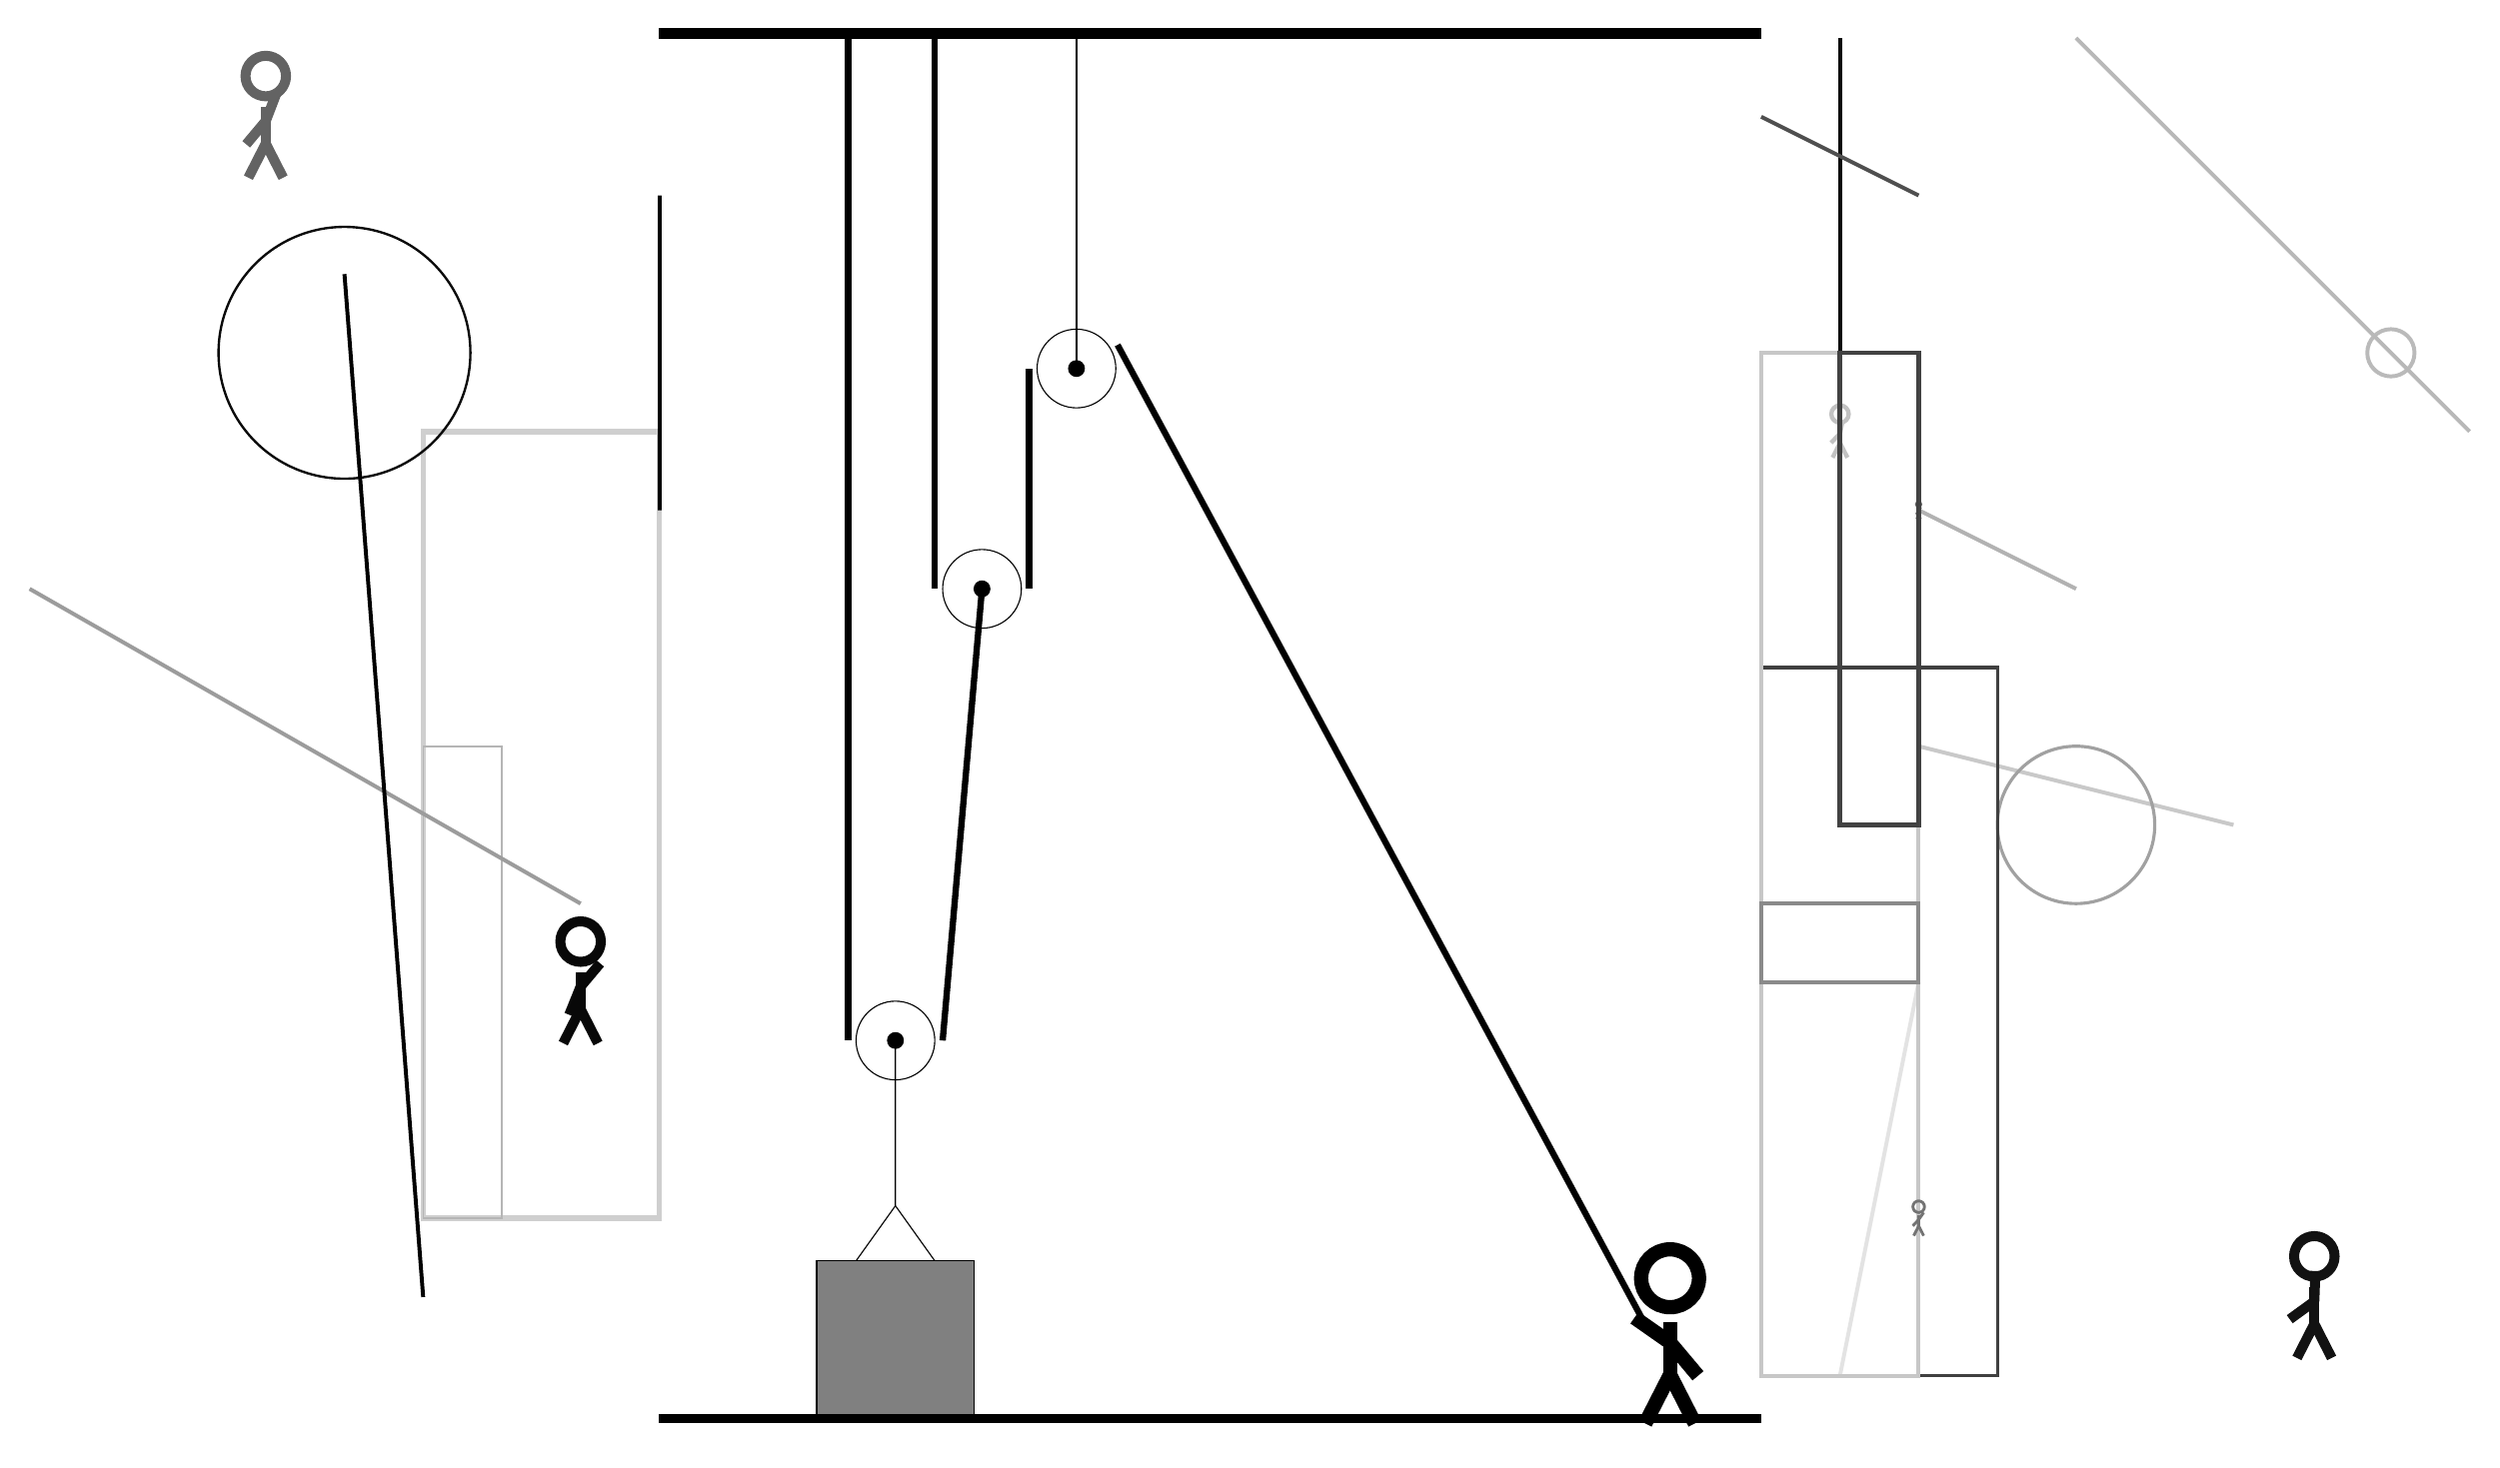
\begin{tikzpicture}
			%%%%% START %%%%%
			
			\draw[fill=black] (-2, 14) rectangle (12, 14.125);
			
			\draw (1, 1.26) circle (0.5);
			\draw[fill=black] (1, 1.26) circle (0.1);
			
			\draw (2.1, 7.0) circle (0.5);
			\draw[fill=black] (2.1, 7.0) circle (0.1);
			
			\draw (3.3, 9.8) circle (0.5);
			\draw[fill=black] (3.3, 9.8) circle (0.1);
			\draw[thick] (3.3, 9.8) -- (3.3, 14);
			
			\draw (1, 1.26) -- (1, -0.84) -- (0.5, -1.54) -- (1.5, -1.54) -- (1, -0.84);
			\draw[fill=black!50] (0, -1.54) rectangle (2, -3.54);
			
			\draw [line width=0.5mm, color=black!27](20, 10) circle (0.3);
			
			\draw[line width=0.7mm, color=black!19] (-2, -1) rectangle (-5, 9);
			\node[line width=0.6mm, color=black!24] at (13, 9) {\Strichmaxerl[3][47][78]};
			\draw[line width=0.2mm, color=black!29] (-4, -1) rectangle (-5, 5);
			
			\node[line width=0.6mm, color=black!93] at (19, -2) {\Strichmaxerl[7][36][88]};
			\node[line width=0.6mm, color=black!97] at (-3, 2) {\Strichmaxerl[7][68][50]};
			
			\draw[line width=0.5mm, color=black!39](-3, 3) -- (-10, 7);
			
			\node[line width=0.2mm, color=black!60] at (14, 8) {\Strichmaxerl[1][49][51]};
			\draw[line width=0.5mm, color=black!30](14, 8) -- (16, 7);
			\draw[line width=0.5mm, color=black!96](13, 4) -- (13, 14);
			\draw[line width=0.5mm, color=black!11](13, -3) -- (14, 2);
			
			\draw[line width=0.5mm, color=black!21](14, 5) -- (18, 4);
			\node[line width=0.5mm, color=black!61] at (-7, 13) {\Strichmaxerl[7][50][69]};
			\draw[line width=0.5mm, color=black!28](16, 14) -- (21, 9);
			\draw [line width=0.4mm, color=black!37](16, 4) circle (1.0);
			\draw[line width=0.4mm, color=black!75] (12, 6) rectangle (15, -3);
			
			\draw[line width=0.5mm, color=black!22] (12, -3) rectangle (14, 10);
			\draw[line width=0.5mm, color=black!46] (14, 3) rectangle (12, 2);
			\draw[line width=0.6mm, color=black!74] (13, 4) rectangle (14, 10);
			\draw [line width=0.3mm, color=black!96](-6, 10) circle (1.6);
			\draw[line width=0.5mm, color=black!100](-6, 11) -- (-5, -2);
			\draw[line width=0.5mm, color=black!100] (-2, 12) rectangle (-2, 8);
			\node[line width=0.2mm, color=black!55] at (14, -1) {\Strichmaxerl[2][47][55]};
			\draw[line width=0.5mm, color=black!69](12, 13) -- (14, 12);
			
			\draw[line width=0.8mm] (0.4, 14) -- (0.4, 1.26);
			\centerarc[line width=0.8mm](1, 1.26)(180:360:0.6);
			\draw[line width=0.8mm](1.6, 1.26) -- (2.1, 7.0);
			\draw[line width=0.8mm] (1.5, 14) -- (1.5, 7.0);
			\centerarc[line width=0.8mm](2.1, 7.0)(180:360:0.6);
			\draw[line width=0.8mm](2.7, 7.0) -- (2.7, 9.8);
			\centerarc[line width=0.8mm](3.3, 9.8)(30:180:0.6);
			\draw[line width=0.8mm] (3.822, 10.1) -- (10.5, -2.3);
			
			\node at (10.8, -2.5) {\Strichmaxerl[10][-35][-50]};
			
			\draw[fill=black] (-2, -3.5) rectangle (12, -3.6);
			
			%%%%% END %%%%%
		\end{tikzpicture}
	\end{figure}	
\end{document}